\section{Lexical Analysis}
\subsection{Regular Expression(正则表达式)}

\begin{figure}[H]
    \centering
    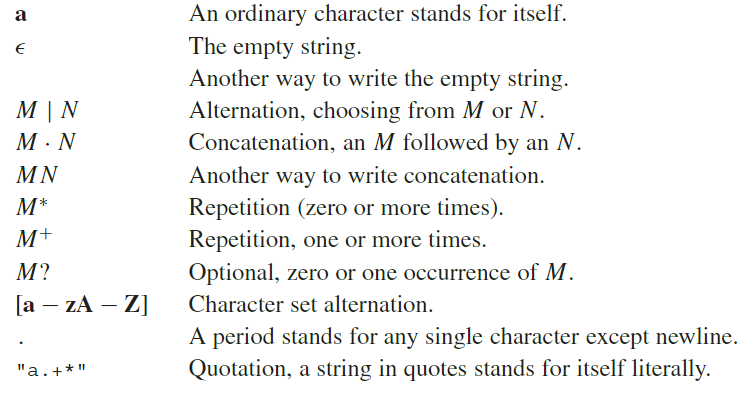
\includegraphics[width=0.88\linewidth]{pic/CP2/Regular expression notation}
    \caption{Regular expression notation}
\end{figure}

优先级: ${}^*> \cdot > |$.

\subsubsection{Two important disambiguation rules}

\begin{enumerate}
    \item 最长匹配
    \subitem 当多个正则表达式都能匹配输入字符串的开头时, 选择匹配最长子字符串的正则表达式. 
    \item 规则优先级
    \subitem 如果最长匹配规则无法解决歧义, 则按照预先定义的优先级顺序选择正则表达式. 
\end{enumerate}

\subsection{Finite Automata}
\begin{itemize}
    \item Deterministic Finite Automaton (DFA) % 看计算理论 II.1-6.
    \item Nondeterministic Finite Automata(NFA)
\end{itemize}

\subsubsection{From a RE to an NFA(naive)}
% 计算理论 III.2 

\subsubsection{From an NFA to a DFA}
% 计算理论 II.13.
$K$ 状态, $\Sigma$ 字符集, $\delta, \Delta$ 转移, $s$ 起始, $F$ 终止. 
\begin{align*}
    \forall&\text{ NFA }M=(K,\Sigma, \Delta, s, F), \\
    \exists&\text{ DFA }M'=(K',\Sigma', \delta', s', F')
\end{align*}
\begin{itemize}
    \item $\Sigma'=\Sigma$
    \item $K'=2^K=\{ Q:Q\subseteq K \}$
    \item $F'=\{ Q\subseteq K:Q\cap F\ne \emptyset \}$
    \item $s'=E(s)$, 
    \subitem $\forall q\in K, E(q)=\{ p\in K:(q,e)\vdash_M^* (p,e) \}$
    \item $\forall Q\subseteq K$, $a\in \Sigma^*$,
    \begin{align*}
        \delta'(Q,a)=\bigcup_{q\in Q}\bigcup_{p:(q,a,p)\in\Delta}E(p)
    \end{align*}
\end{itemize}
$E(q)$(闭包)相当于在 $q$ 零步之内(不耗费输入的字符)能到达的结点.  $\delta'(Q,a)$ 相当于 $Q$ 中每个状态 $q$ 接受 $a$ 到达 $p$ 后, 所有 $p$ 闭包的并集. 


% \begin{example}
% NFA:

% \begin{tikzpicture}[shorten >=1pt, node distance=2cm, on grid, auto]
%     \node[state,initial]  (q_0)                      {$q_0$};
%     \node[state, accepting] (q_1) [right=of q_0] {$q_1$};

%     \path[->] (q_0) edge node {b} (q_1)
%                     edge [loop above] node {a} ()
%               (q_1) edge [bend left] node  {e} (q_0)
%             ;
% \end{tikzpicture}

% DFA:

% \begin{tikzpicture}[shorten >=1pt, node distance=2cm, on grid, auto]
%     \node[state,initial]  (q_0)                      {$\{q_0\}$};
%     \node[state, accepting] (q_1) [below=of q_0] {$\{q_1\}$};
%     \node[state, accepting] (q_0q_1) [right=of q_0] {$\{q_0, q_1\}$};
%     \node[state] (empty) [right=of q_1] {$\emptyset$};

%     \path[->] (q_0) edge [bend left] node {b} (q_0q_1)
%                     edge [loop above] node {a} ()
%               (q_0q_1) edge [bend left] node {a} (q_0)
%                        edge [loop right] node {b} ()
%                 (q_1) edge node {a,b} (empty)
%             ;
% \end{tikzpicture}

% $\{q_1\}$ 与 $\emptyset$ 可省略. 
% \end{example}

\subsubsection{The equivalent states}
Hopcroft’s algorithm: 通过寻找合并等价状态对, 构造最简 DFA. 

